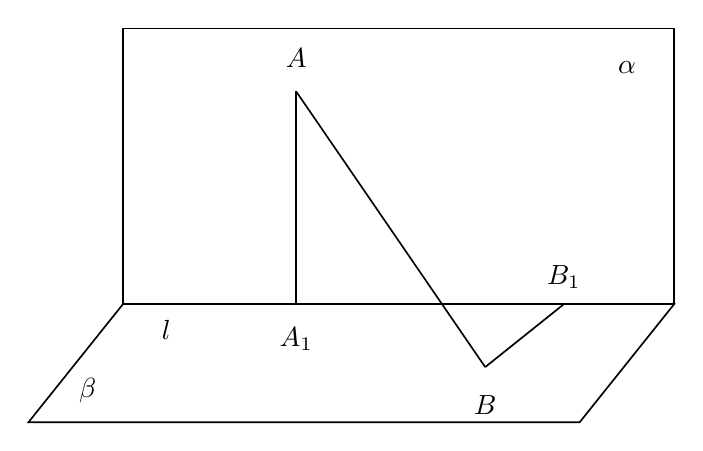
\begin{tikzpicture}[x=1cm,y=1cm,line width=.6pt,font=\normalsize,
  geometry edge/.style={solid,line width=.6pt},
  geometry label/.style={font=\normalsize,inner sep=2pt}]
% Intersecting planes alpha (top rectangle) and beta (bottom parallelogram).
% l is the horizontal intersection line y=1.5.
% A in alpha with foot A1 on l; B in beta with foot B1 on l.
\coordinate (L0) at (0,1.5);
\coordinate (L1) at (7,1.5);
\coordinate (Atr) at (7,5);
\coordinate (Atl) at (0,5);
\coordinate (Rb2) at (5.8,0);
\coordinate (Lb2) at (-1.2,0);
\coordinate (A) at (2.2,4.2);
\coordinate (A1) at (2.2,1.5);
\coordinate (B1) at (5.6,1.5);
\coordinate (B) at (4.6,0.7);
% Plane outlines (solid), l drawn as shared edge
\draw[geometry edge] (L0)--(L1)--(Atr)--(Atl)--cycle;
\draw[geometry edge] (L0)--(L1)--(Rb2)--(Lb2)--cycle;
% Interior segments
\draw[geometry edge] (A)--(A1);
\draw[geometry edge] (A)--(B);
\draw[geometry edge] (B1)--(B);
% Labels placed clear of all strokes
\node[geometry label,anchor=south] at (2.2,4.42) {$A$};
\node[geometry label,anchor=north] at (2.2,1.28) {$A_{1}$};
\node[geometry label,anchor=south] at (5.6,1.62) {$B_{1}$};
\node[geometry label,anchor=north] at (4.6,0.42) {$B$};
\node[geometry label,anchor=north] at (0.55,1.38) {$l$};
\node[geometry label,anchor=center] at (6.4,4.5) {$\alpha$};
\node[geometry label,anchor=center] at (-0.45,0.4) {$\beta$};
\end{tikzpicture}
